\documentclass[12pt,letterpaper]{report}
\usepackage[utf8]{inputenc}
\usepackage[spanish,es-tabla]{babel}
\usepackage{amsmath}
\usepackage{amsfonts}
\usepackage{amssymb}
\usepackage{physics}
%\usepackage{cite}
\usepackage{graphicx}
\DeclareGraphicsExtensions{.png,.jpg}
\usepackage[table]{xcolor}
%\usepackage[usenames]{color}
\usepackage[draft,inline,nomargin]{fixme} \fxsetup{theme=color}
\FXRegisterAuthor{cc}{acc}{\color{green}CC}
\usepackage{wrapfig}
\usepackage{multirow}
\usepackage{hyperref}
\usepackage{booktabs}
\usepackage[backend=bibtex,style=phys]{biblatex}
\bibliography{referencias}
\usepackage[left=2.5cm,right=2.5cm,top=2cm,bottom=2cm]{geometry}
\usepackage{setspace}

\begin{document}
\chapter{Resultados}
\spacing{1.25}

%Introduccion del capítulo
En este cap\'itulo se discuten los resultados obtenidos de las simulaciones de cascadas atmosf\'ericas. Se realiza un ajuste de la distribuci\'on lateral de muones a una funci\'on de tipo NKG modificada, y se grafican los par\'ametros del ajuste en funci\'on de la energ\'ia primaria. Se comparan los par\'ametros obtenidos como resultado de distintas part\'iculas primarias, diferentes modelos de interacciones hadr\'onicas y distintos \'angulos de incidencia.

\section{Distribuci\'on lateral de muones}
- Generalidades de qu\'e se esperaba  de las distribuciones laterales, comparando protones y hierro.

	\begin{figure}[H] \label{fig:lateraldist}
	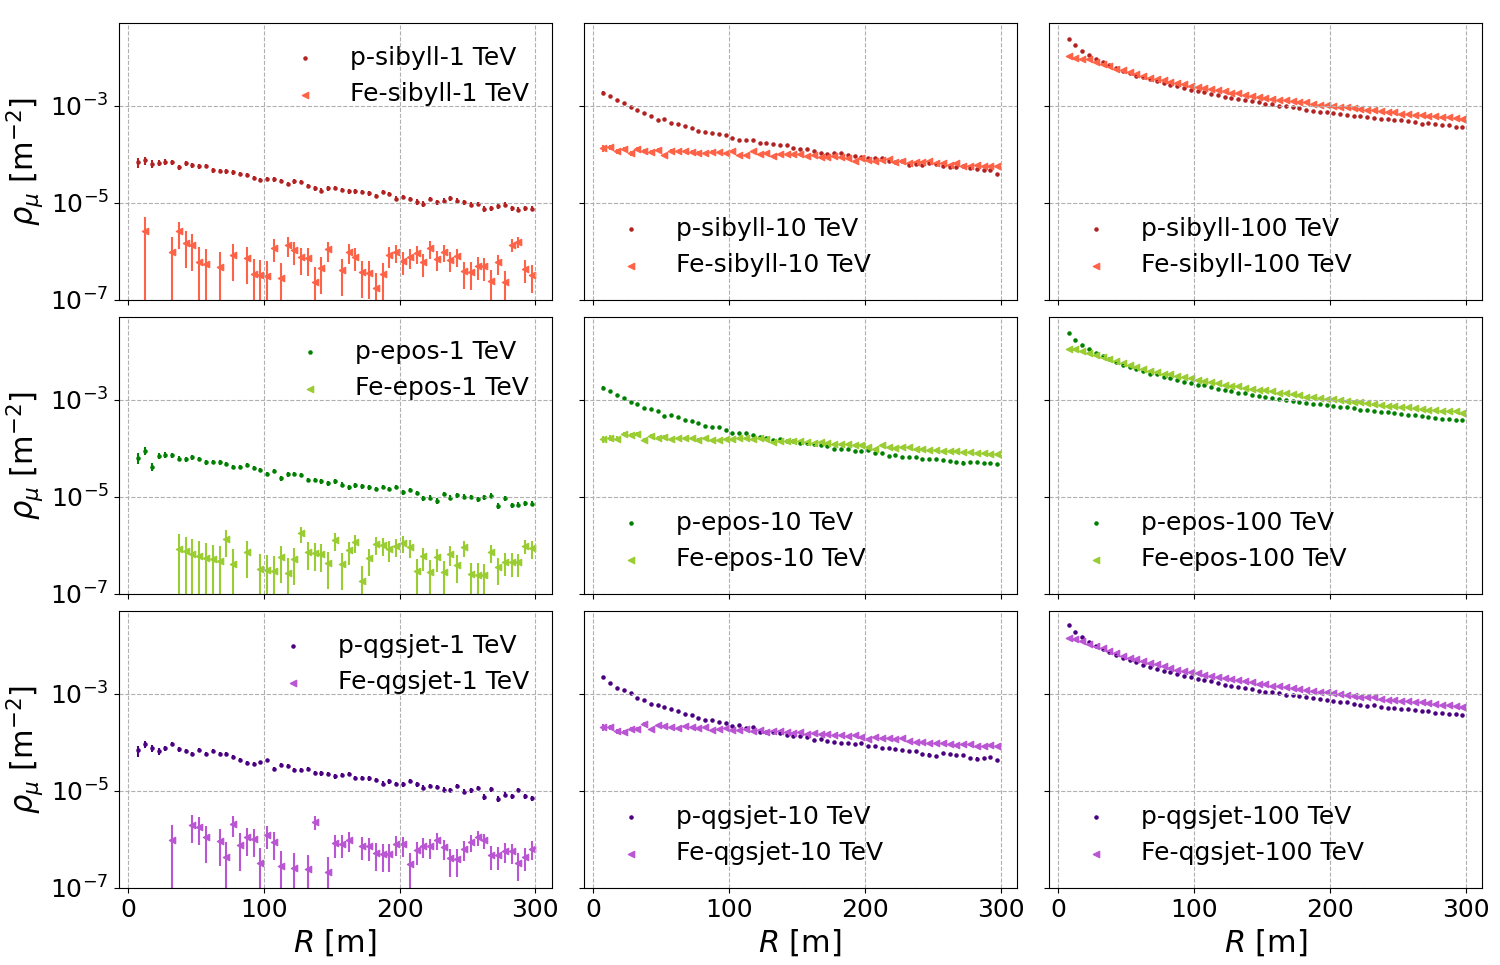
\includegraphics[width=\textwidth]{Figuras/lateraldist}
	\end{figure}

	\subsection{Ajustes a una funci\'on de tipo NKG}
	- Presentaci\'on de la funci\'on y justificarla. (Cita a Malone2018).
	- Interpretaci\'on de los par\'ametros libres.
	
		\begin{figure}[H] \label{fig:lateraldist_wfits}
		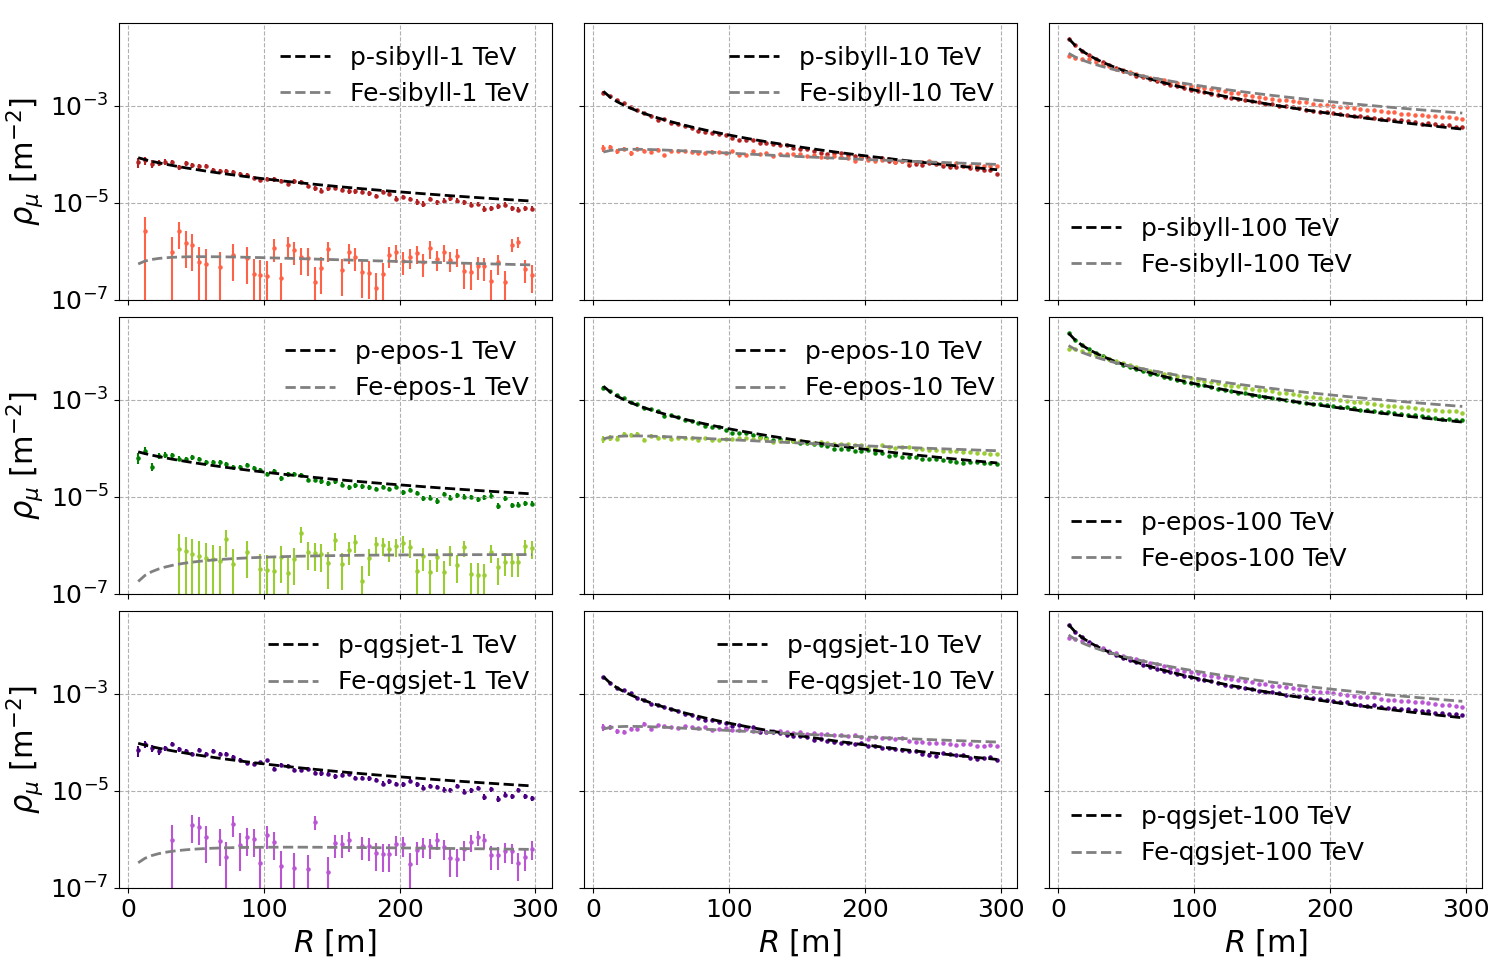
\includegraphics[width=\textwidth]{Figuras/lateraldist_wfits}
		\end{figure}
		
\section{Par\'ametros del ajuste}

	\subsection{Modelos de interacciones hadr\'onicas}
	\subsection{Composici\'on primaria}
	\subsection{\'Angulo de incidencia}
	\ccnote{puedo sacar tambi\'en los par\'ametros en funci\'on de theta, aunque estar\'ia alguito complicado}
		\begin{figure}[H] \label{fig:theta_nkgA}
		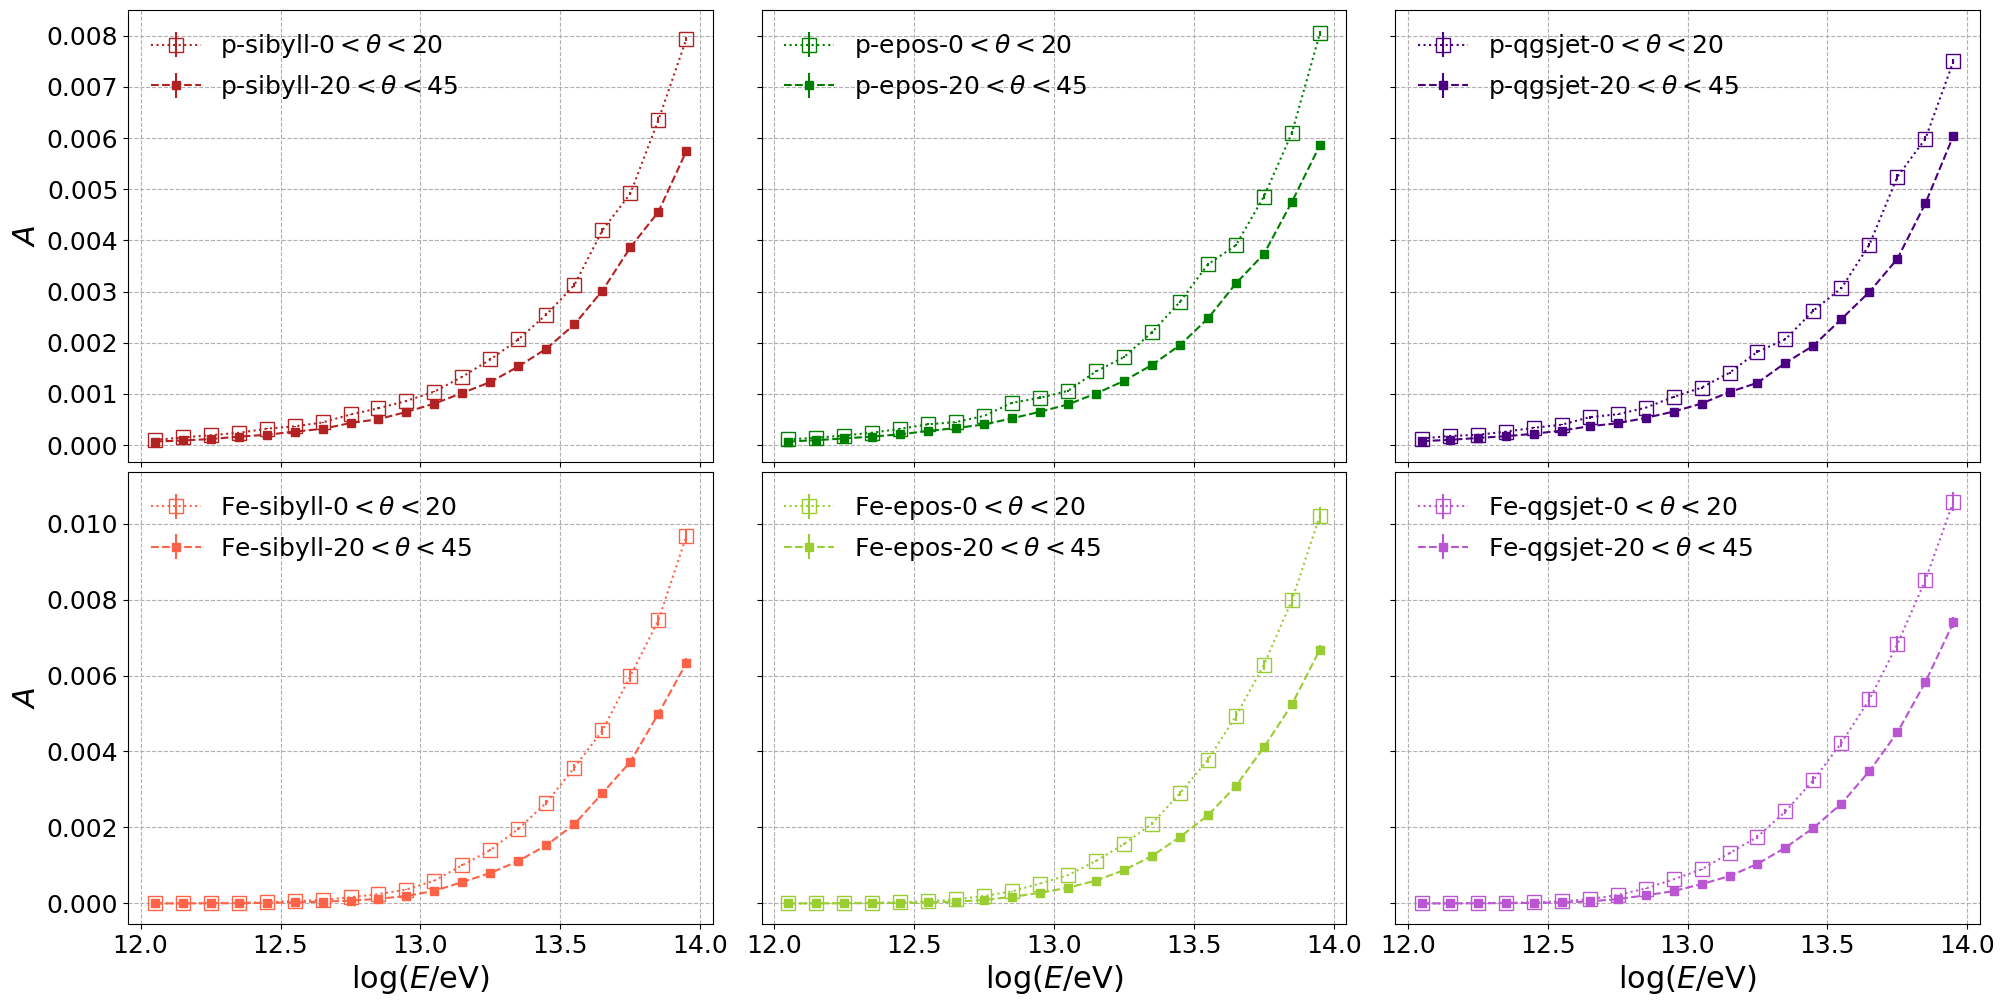
\includegraphics[width=\textwidth]{Figuras/theta_nkgA}
		\end{figure}
		
		\begin{figure}[H] \label{fig:theta_nkgs}
		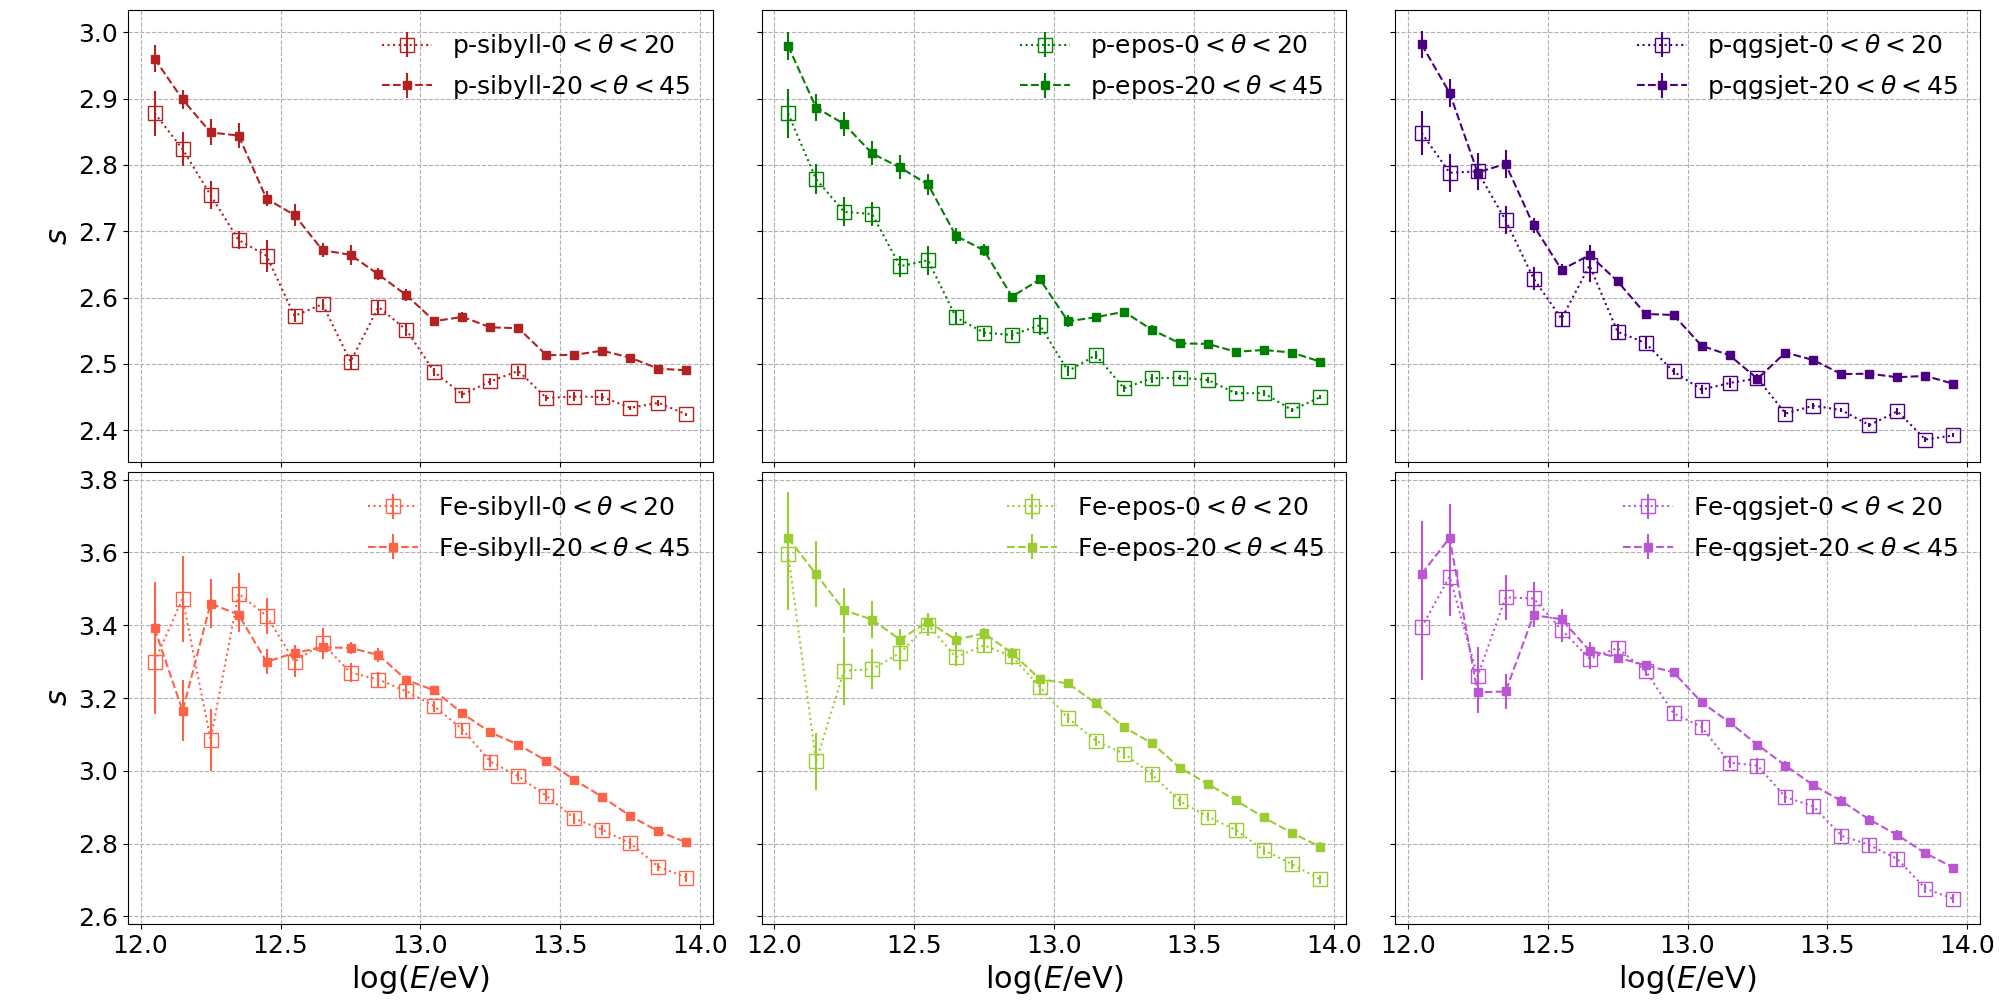
\includegraphics[width=\textwidth]{Figuras/theta_nkgs}
		\end{figure}

\singlespacing
\end{document}